\chapter{Layout Guidelines for a Activity Flow Diagram}
\label{chp:af:layout}

\section{Introduction}

The previous chapters describe the appearance and meaning of
\SBGNAFLone components. Objects are \glyph{AFNs}, \glyph{container nodes}, 
\glyph{logical operators} as well as \glyph{connecting arcs}. 
The components of a \AF have to be placed in a meaningful way -- a random
distribution with spaghetti-like connections will most likely hide
the information encoded in the underlying model, whereas an elegant
placement of the objects, giving a congenial appearance of the
diagrams, may reveal new insights. The arrangement of components in a
diagram is called a \emph{layout}.

SBGN \AFs should be easily recognisable not only by the
glyphs used, but also by the general style of the layout. However, the
arrangement of the components is a complex art in itself, and there is
no simple rule which can be applied to all cases. Therefore this
section provides guidelines for the layout of process diagrams, divided
into two categories:
\begin{enumerate}
  \item requirements, \ie rules which \textbf{must} be fulfilled by a
  layout, and
  \item recommendations, \ie rules which \textbf{should} be followed if
  possible.
\end{enumerate}
In addition, we provide a list of additional suggestions which may help in 
producing aesthetically more pleasant layouts, possibly easier to understand.

Those layout guidelines are independent of the method used to produce
the diagram, and apply to both manually drawn diagrams as well as
diagrams produced by an automatic layout algorithm. The guidelines do
not deal with interactive aspects (\eg the effect of zooming). 
Further information about automatic network layout
(graph drawing) can be found, for example, in the books of Di Battista and
co-authors~\cite{DiBattista:1998} and Kaufmann and Wagner~\cite{Kaufmann:2001}.

Please note that the color of objects do not carry any meaning in
SBGN. Although one can use colors to emphasize part of a diagram or
encode additional information, the meaning of the diagram should not
depend on the colors. Furthermore, objects can have different sizes
and size is also meaningless in SBGN. For example, a transition node
may be larger than a protein node. Also the meaning of a graph
should be conserved upon scaling as far as possible.

\newpage

\section{Layout guidelines}

\subsection{Requirements}

Requirements are rules which \textbf{must} be fulfilled by a layout to
produce a valid \SBGNAFLone graph.

\subsubsection{Node-node overlaps}
\label{af:NoNoOv}

Nodes are only allowed to overlap in two cases:
\begin{enumerate}
  \item the overlapping nodes define a glyph (\eg a \glyph{multimer}
  composed by stacking of two containers representing the monomers).
  \item nodes overlapping compartments
  (\eg a complex placed on the compartment border).
\end{enumerate}
Otherwise, nodes are not allowed to overlap (\fig{af:layout1}). This includes the
touching of nodes. Touching is not allowed apart from the case where
it has a specific meaning, \eg two macromolecules touching each
other within a complex because they form the complex. Submaps
are not allowed to overlap.

\begin{figure}[h!]
  \centering
  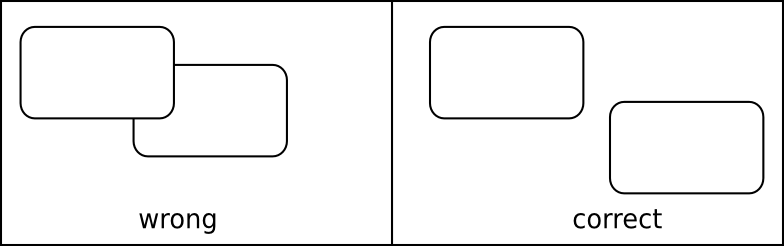
\includegraphics[scale=0.3]{images/layout-node-node}
  \caption{Nodes must not overlap.}\label{fig:af:layout1}
\end{figure}

\subsubsection{Node-edge crossing}
\label{af:crosEdNoRe}

In case of node-edge crossing the edge must be drawn on the top of
the node (\fig{af:layout2}). See also recommendation \ref{af:crosEdNo} (crossing between
edges and nodes should be avoided).

\begin{figure}[h!]
  \centering
  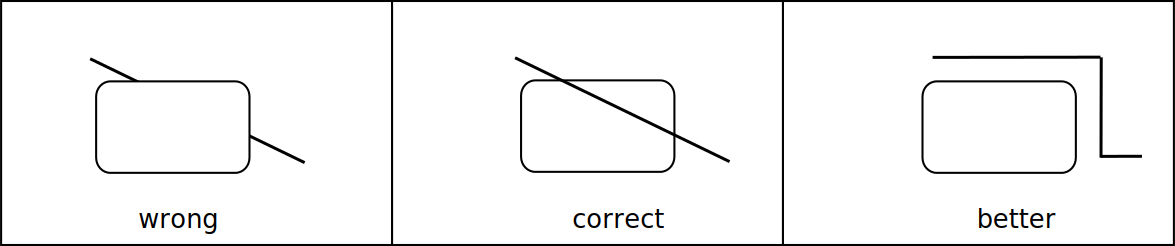
\includegraphics[scale=0.3]{images/layout-node-edge}
  \caption{If an edge crosses a node, the edge must be drawn on top
  of the node.}\label{fig:af:layout2}
\end{figure}

\subsubsection{Node border-edge overlaps}

Edges are not allowed to overlap the border lines of nodes (\fig{af:layout3}).

\begin{figure}[h!]
  \centering
  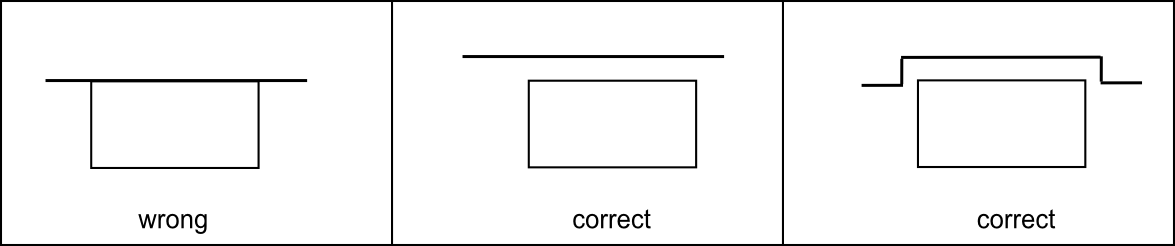
\includegraphics[scale=0.3]{images/layout-node-border-edge}
  \caption{Edges must not overlap node borders.}\label{fig:af:layout3}
\end{figure}

\subsubsection{Edge-edge overlaps}

Edges are not allowed to overlap (\fig{af:layout4}). This includes touching of edges.
Furthermore, an edge is neither allowed to cross itself nor to cross
a boundary of node more than twice or other edges more than once.

\begin{figure}[h!]
  \centering
  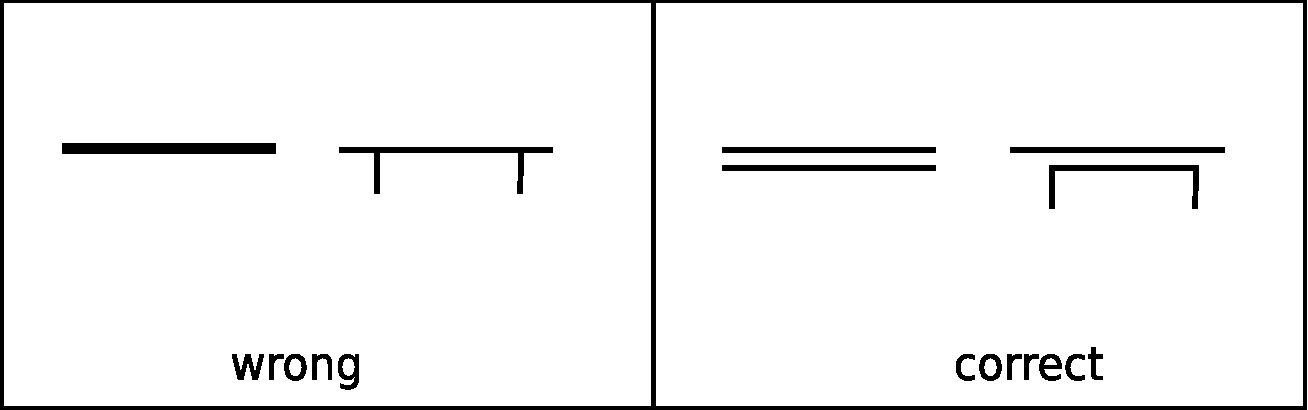
\includegraphics[scale=0.3]{images/layout-edge-edge}
  \caption{Edges must not overlap.}\label{fig:af:layout4}
\end{figure}

\subsubsection{Node orientation}

Nodes have to be drawn horizontally or vertically, any other
rotation of elements is not allowed (\fig{af:layout5}).

\begin{figure}[h!]
  \centering
  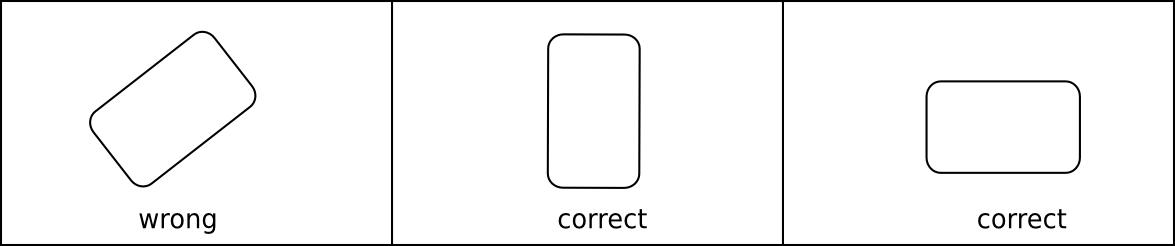
\includegraphics[scale=0.3]{images/layout-orientation}
  \caption{The node orientation must be horizontally or
  vertically.}\label{fig:af:layout5}
\end{figure}

\subsubsection{Node-edge connection}

The arcs linking the square glyph of a \glyph{transition} 
to the \glyph{consumption} and \glyph{production arcs}
are attached to the center of opposite sides (\fig{af:layout6}). 
The modulatory arcs are attached to the other two sides, but not necessarily
all to the center, as several modifiers can affect the same \glyph{transition
node}. A \glyph{transition} connected to \glyph{production arcs} on opposite
sides is a reversible transition.

\begin{figure}[h!]
  \centering
  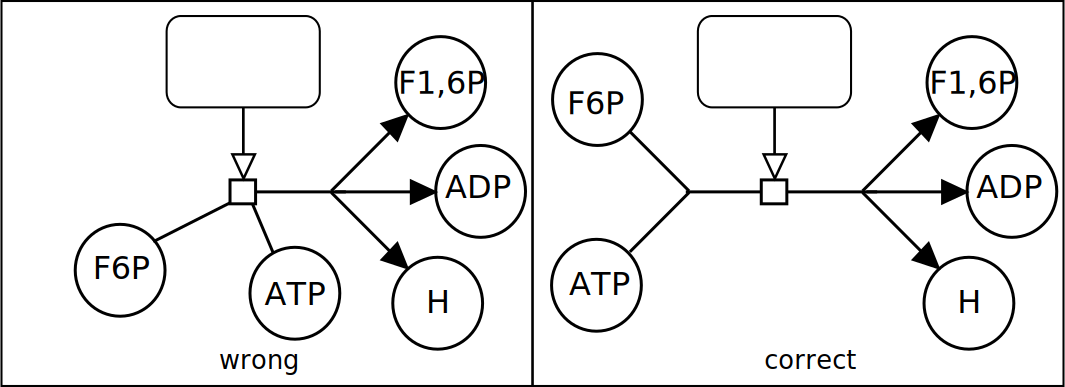
\includegraphics[scale=0.3]{images/layout-connecting-arcs}
  \caption{Arcs between a \glyph{transition}  and the 
  \glyph{consumption} and \glyph{production arcs} must be attached 
  to the center of opposite sides, modulatory
  arcs must be attached to the other two sides.}\label{fig:af:layout6}
\end{figure}

\subsubsection{Node labels}

At least a part of the label (unbordered box containing a string of
characters) has to be placed inside the node it belongs to. Node
labels are not allowed to overlap nodes or other labels (this
includes touching of other nodes or labels).

\subsubsection{Edge labels}

Edge labels are not allowed to overlap nodes. This includes touching
of nodes.

\subsubsection{Compartments}

If a transition has all participants in the same compartment the
transition node and all edges/arcs have to be in this compartment.
If a transition has participants in at least two different
compartments, the transition node has to be either in a compartment
where the transition has at least one participant or in the empty
space.

\subsection{Recommendations}

Recommendations are rules which should be followed if possible to
produce layouts may be easier to understand.

\subsubsection{Node-edge crossing}
\label{af:crosEdNo}

Crossings between edges and nodes should be avoided. Some crossings
may be unavoidable, \eg the crossing between an edge and a
compartment border or an edge and a complex (if the edge connects an
element inside the complex with something outside). See also
requirement \ref{af:crosEdNoRe} (in case of node-edge crossings the
edge must be drawn on the top of the node).

\subsubsection{Labels}

Labels should be horizontal. Node labels should be placed completely
inside the node if possible.3 Edge labels should be placed close to
the edge and avoid overlapping the edge as well as other edge
labels.

\subsubsection{Avoid edge crossings}

The amount of crossings between edges should be minimized.

\subsubsection{Branching of \glyph{association} and \glyph{dissociation}}

The branching points of \glyph{association} and \glyph{dissociation} nodes 
should be placed closed to the symbol of the transition, if possible 
at a distance comparable than, or smaller to, the diameter of the 
symbol defining the transition (\fig{af:branching}).

\begin{figure}[h!]
  \centering
  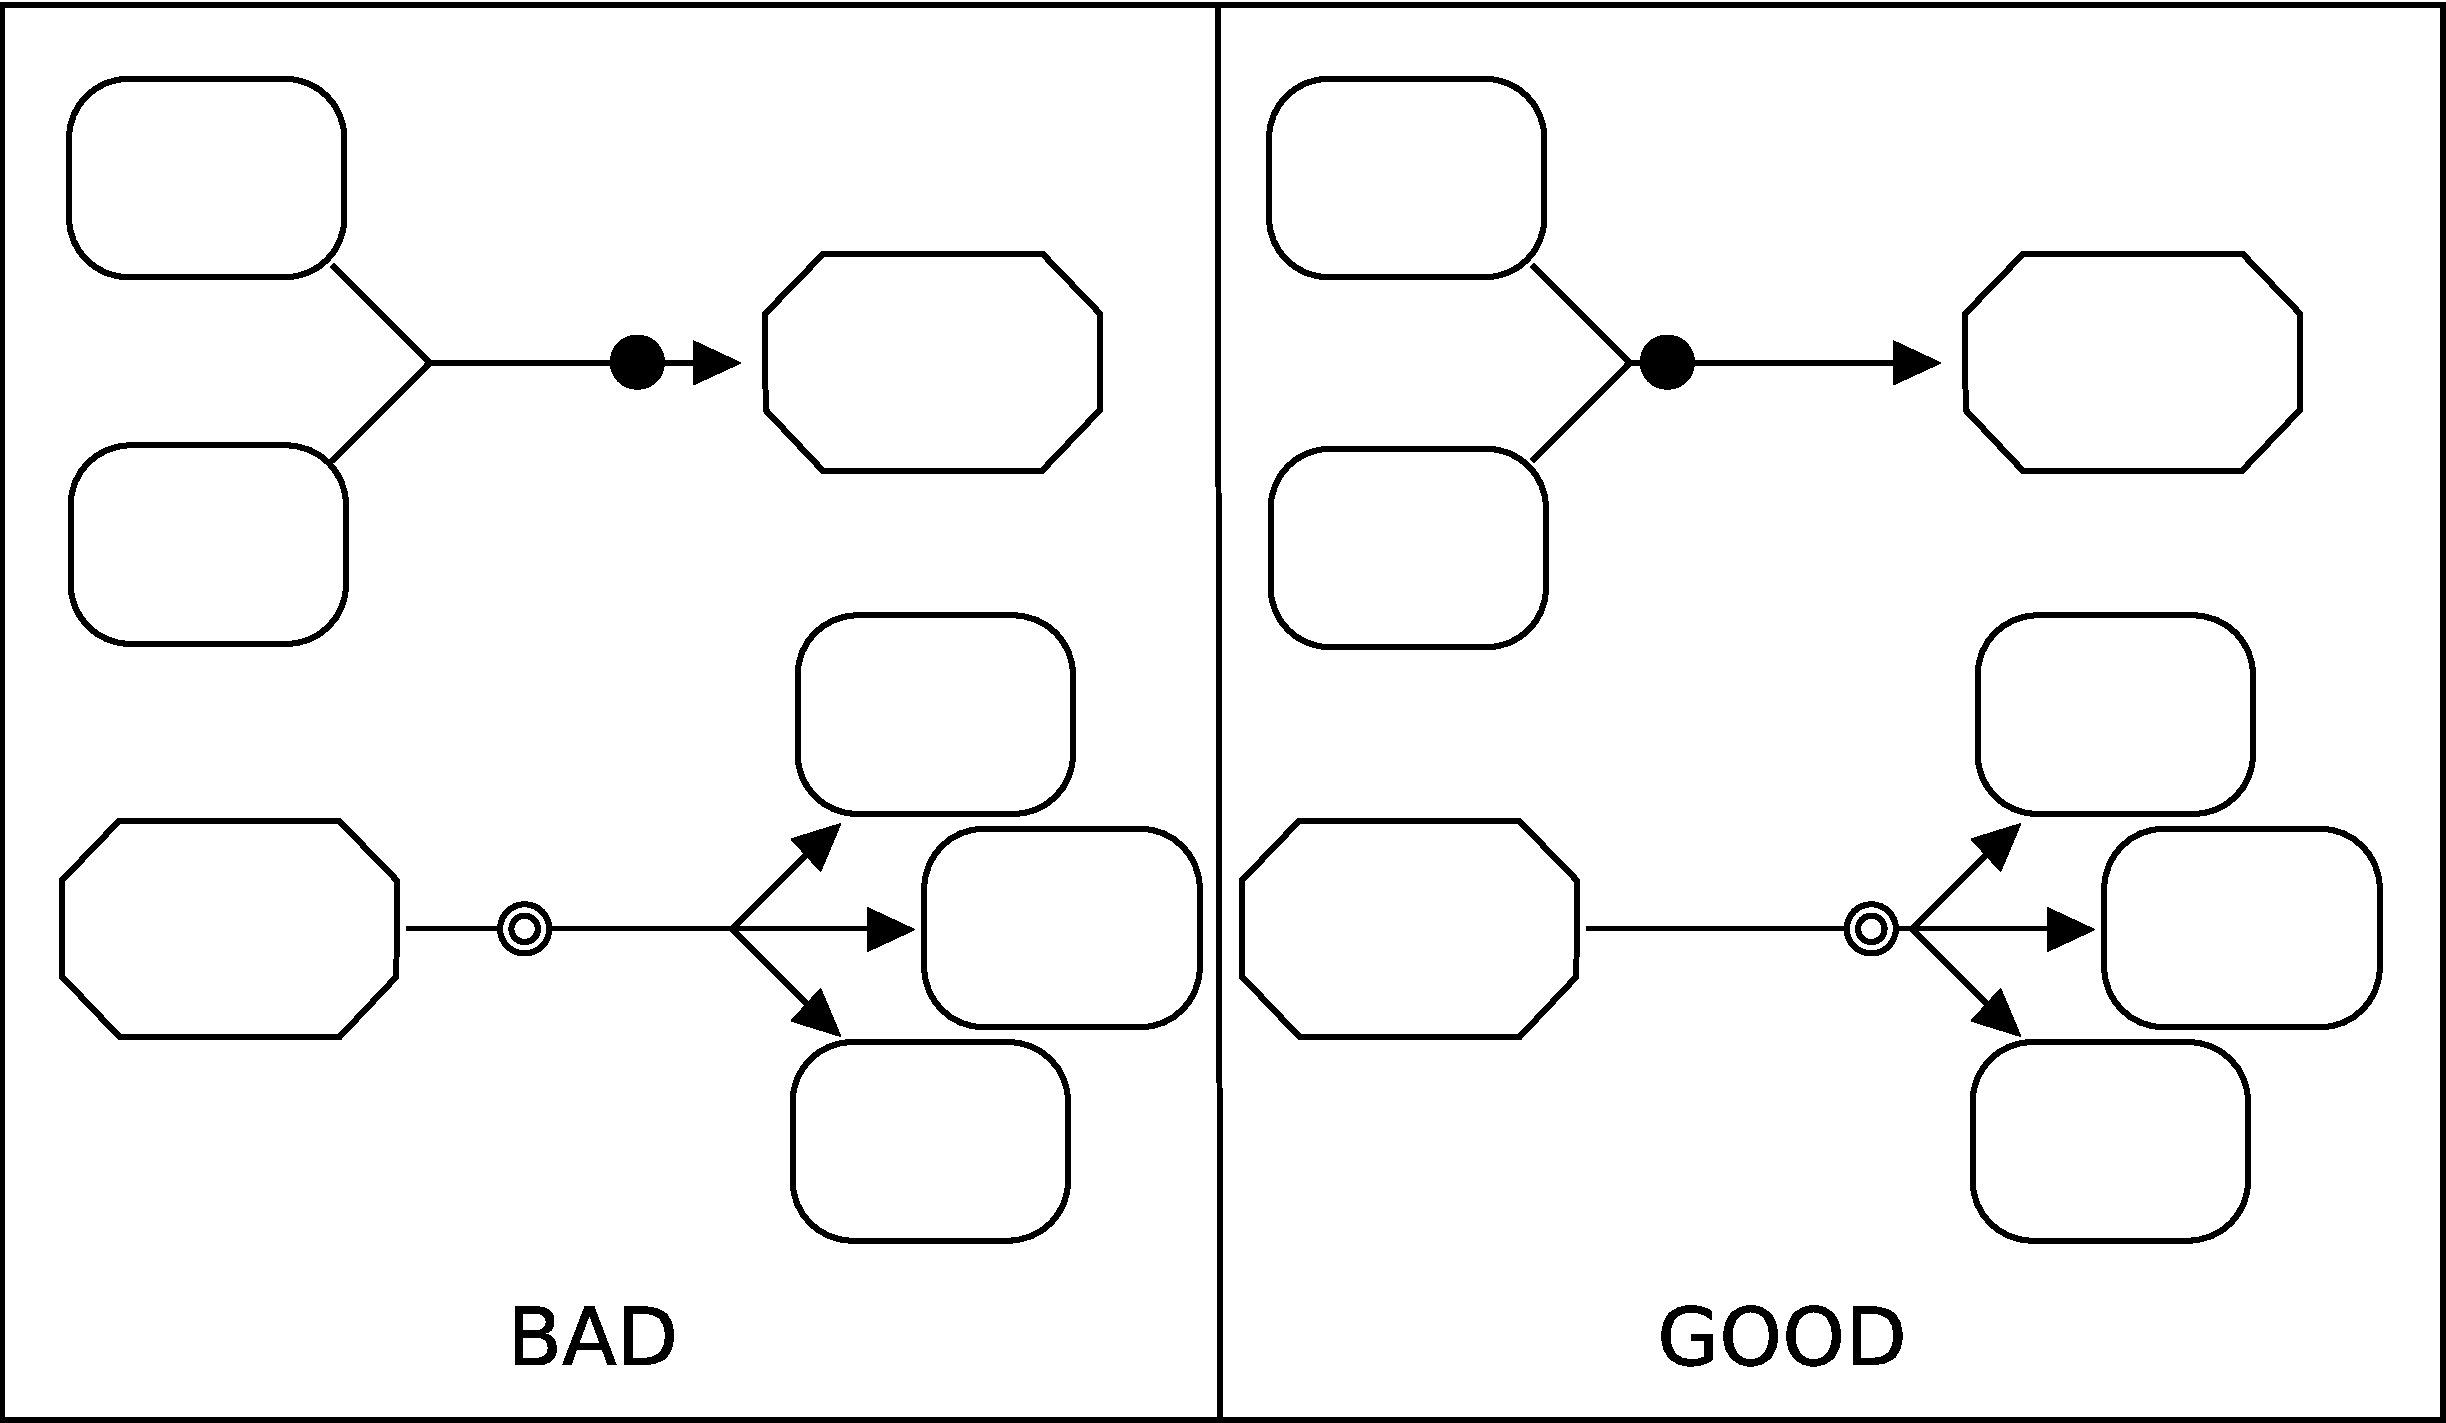
\includegraphics[scale=0.3]{images/layout-branching}
  \caption{Branching points should be close to association and 
  dissociation symbols.}\label{fig:af:branching}
\end{figure}

\subsubsection{Units of information}

Units of information should not hide the structure of the
corresponding node and should not overlap other
elements (\fig{af:layout7}).

\begin{figure}[h!]
  \centering
  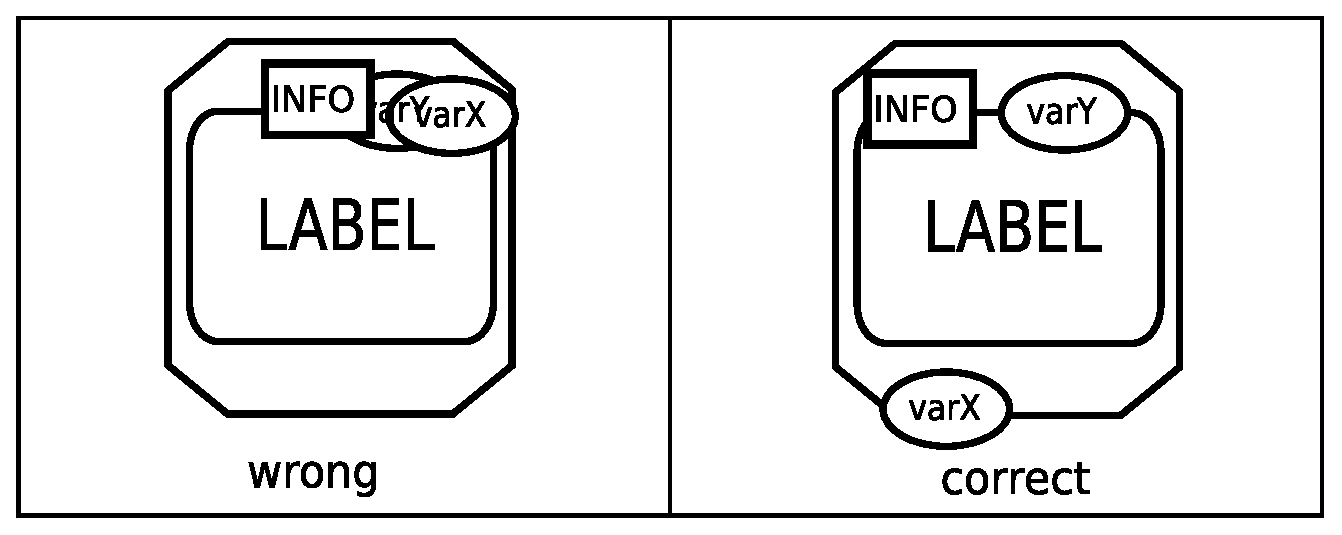
\includegraphics[scale=0.5]{images/layout-unit-information}
  \caption{Units of information should not overlap with any
  other element.}\label{fig:af:layout7}
\end{figure}

\subsection{Additional suggestions}

Here is a list of additional layout suggestions which may help in
producing aesthetically more pleasing layouts which may be easier to
understand.

\begin{itemize}
  \item Angle of edge crossings: If edge crossings are not avoidable
  edges should cross with an angle close to 90 degrees.
  \item Placement of substrates and products of a transition:
  Substrate and product nodes should be placed
  on different sides of the transition node.
  \item Drawing area and width/height ratio: The drawing should
  be compact and the ratio between the width and the height
  of the drawing should be close to 1.
  \item Edge length: Long edges should be avoided.
  \item Number of edge bends: Edges should be drawn with
  as few bends as possible.
  \item Similar and symmetric parts: Similar parts of a diagram
  should be drawn in a similar way, and symmetric parts
  should be drawn symmetrically.
  \item Proximity information: Related elements (\eg nodes
  connected by a transition or all elements within a compartment)
  should be drawn close together.
  \item Directional information: Subsequent processes (\eg a sequence
  of reactions) should be drawn in one direction (\eg from
  top to bottom or from left to right).
  \item Compartments: Different compartments should have different
  background shade or color.
\end{itemize}
